\subsubsection{La fonction tangente: tan(x)}
La tangente d'un angle $\alpha$ dans un triangle rectangle est définie comme
le rapport entre la longueur du côté opposé à cet angle et la
longueur du côté adjacent. Si on note $h$ la longueur de l'hypoténuse,
$a$ la longueur du côté adjacent à $\alpha$ et $o$ la longueur du côté
opposé on a :
\[
  \tan(\alpha) = \frac{o}{a} = \frac{\frac{o}{h}}{\frac{a}{h}} =
  \frac{sin(\alpha)}{\cos(\alpha)}
\]

\textbf{Problème: } Que se passe t'il quand $\alpha = \frac{\pi}{2} +
k\pi$ pour $k \in \mathbb{Z}$. La tangente n'est pas défini en ces
points.

Ainsi on défini la fonction trigonométrique tangente de la manière
suivante:

\begin{center}
  $\begin{array}{cccccc}
     f & : & \R \backslash \{ \frac{pi}{2} + k \pi \} & \to & \R, &
       k \in \mathbb{Z}\\
       & & x & \mapsto & \tan(x)=\frac{sin(x)}{cos(x)} \\
   \end{array}$
 \end{center}

\textbf{Propriétés de la fonction tangente: }
\begin{itemize}[label=$\bullet$, leftmargin=2cm]
\item $\tan$ est continue sur chaque intervalle de la forme
  $[(2k+1)\frac{\pi}{2}, (2k+1)\frac{\pi}{2} + \pi],~ k \in \mathbb{Z}$
\item $\tan$ est dérivable sur chaque intervalle de la forme
  $[(2k+1)\frac{\pi}{2}, (2k+1)\frac{\pi}{2} + \pi]$ et $\tan'(x)
  =\frac{1}{cos^2(x)} = 1+tan^2(x)$ (A montrer)
\item $\tan$ est croissante sur chaque intervalle de la forme
  $[(2k+1)\frac{\pi}{2}, (2k+1)\frac{\pi}{2} + \pi]$ 
\item $\tan(x+2k\pi) = tan(x),~ k \in \mathbb{Z}$ (2-$\pi$
  périodique)
\item $\lim \limits_{x \to -\frac{\pi}{2}^+} tan(x) = -\infty$ et $\lim
  \limits_{x \to \frac{\pi}{2}^-} tan(x) = \infty$ 
\end{itemize}

\vspace{1\baselineskip}

\hspace{-2.5cm}
\begin{minipage}{0.4\linewidth}
  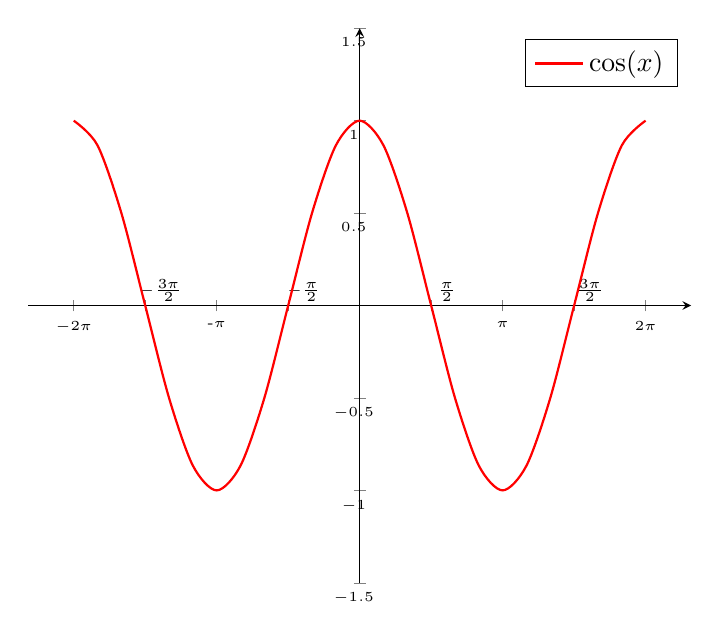
\begin{tikzpicture}
    \begin{axis}[
      width = 10cm,
      xmin = -2*pi-1,
      xmax = 2*pi+1 ,
      ymin = -1.5,
      ymax = 1.5,
      axis x line= center,
      axis y line= center,        
      xtick=
      {-6.28318,-3.14159, 0, 3.14159, 6.28318},
      ticklabel style={font = \tiny, below},
      xticklabels =
      {$-2\pi$,-$\pi$,$0$,$\pi$,$2\pi$},
      extra x ticks = {-4.7123889, -1.5708, 1.5708, 4.7123889},
      extra x tick labels =
      {$-\frac{3\pi}{2}$,$-\frac{\pi}{2}$,$\frac{\pi}{2}$,$\frac{3\pi}{2}$},
      extra x tick style={tick label style={above, xshift=0.2cm}}
      ]
      \addplot[mark=none, domain = -2*pi:2*pi, red, smooth, thick]
      {cos(deg(x))};
      \legend{$\cos(x)$}
    \end{axis}
  \end{tikzpicture}
\end{minipage}
\hspace{4cm}
\begin{minipage}{0.4\linewidth}
  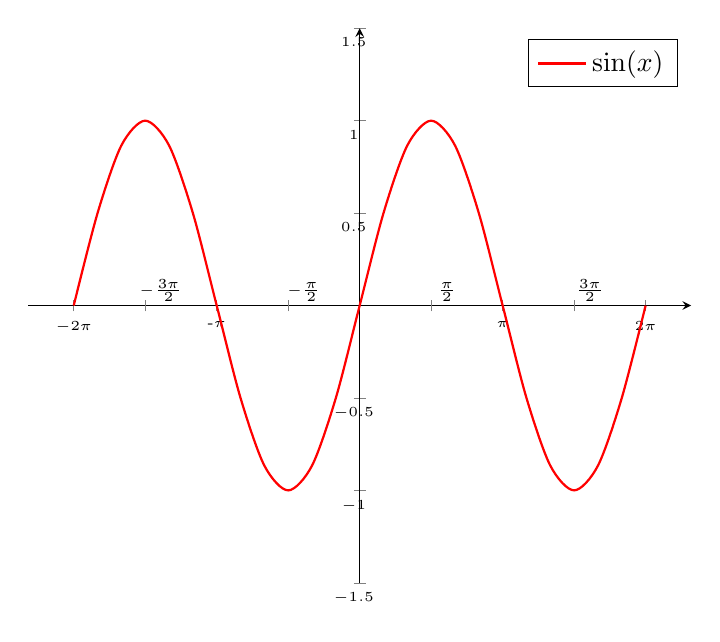
\begin{tikzpicture}
    \begin{axis}[
      width = 10cm,
      xmin = -2*pi-1,
      xmax = 2*pi+1 ,
      ymin = -1.5,
      ymax = 1.5,
      axis x line= center,
      axis y line= center,        
      xtick=
      {-6.28318,-3.14159, 0, 3.14159, 6.28318},
      ticklabel style={font = \tiny, below},
      xticklabels =
      {$-2\pi$,-$\pi$,$0$,$\pi$,$2\pi$},
      extra x ticks = {-4.7123889, -1.5708, 1.5708, 4.7123889},
      extra x tick labels =
      {$-\frac{3\pi}{2}$,$-\frac{\pi}{2}$,$\frac{\pi}{2}$,$\frac{3\pi}{2}$},
      extra x tick style={tick label style={above, xshift=0.2cm}}
      ]
      \addplot[mark=none, domain = -2*pi:2*pi, red, smooth, thick]
      {sin(deg(x))};
      \legend{$\sin(x)$}
    \end{axis}
  \end{tikzpicture}
\end{minipage} 

\begin{center}
  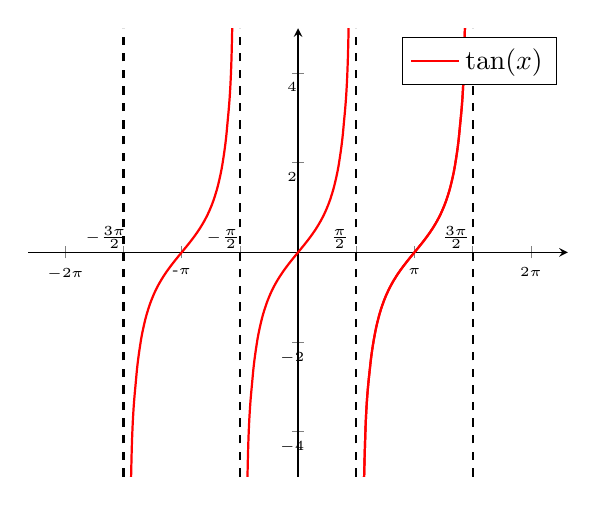
\begin{tikzpicture}
    \begin{axis}[
      xmin = -2*pi-1,
      xmax = 2*pi+1 ,
      ymin = -5,
      ymax = 5,
      axis x line= center,
      axis y line= center,        
      xtick=
      {-6.28318,-3.14159, 0, 3.14159, 6.28318},
      ticklabel style={font = \tiny, below},
      xticklabels =
      {$-2\pi$,-$\pi$,$0$,$\pi$,$2\pi$},
      extra x ticks = {-4.7123889, -1.5708, 1.5708, 4.7123889},
      extra x tick labels =
      {$-\frac{3\pi}{2}$,$-\frac{\pi}{2}$,$\frac{\pi}{2}$,$\frac{3\pi}{2}$},
      extra x tick style={tick label style={above, xshift=-0.21cm}}
      ]
      \addplot [mark=none, domain = -pi/2+0.1:pi/2-0.1, red, smooth, thick]
      {tan(deg(x))};
      \addplot [mark=none, domain = -3*pi/2+0.1:-pi/2-0.1, red, smooth, thick]
      {tan(deg(x))};
      \addplot [mark=none, domain = pi/2:3*pi/2-0.1, red, smooth, thick]
      {tan(deg(x))};
      \addplot [mark=none, domain = pi/2:3*pi/2-0.1, red, smooth, thick]
      {tan(deg(x))};
      \foreach \k in {-3,-1,...,3}
      {
        \addplot[dashed, thick, smooth, black] coordinates
        {(\k*pi/2,-5)(\k*pi/2,5)};
      }
      \legend{$\tan(x)$}
    \end{axis}
  \end{tikzpicture}
\end{center}

\subsection{Les fonctions trigonométriques réciproques}
\subsubsection{L'arccosinus: $\arccos(x)$}

L'arc cosinus d'un nombre réel compris entre -1 et 1 est la ``mesure principale
de l'angle'' dont le cosinus vaut ce nombre, ``compris entre  $0$ et
$\pi$). (Montrer qu'on a bijection sur cet intervalle ? Parler de $cos^{-1}$ sur
les calculatrices)

Cette fonction est alors la fonction réciproque de la fonction cosinus définie
sur l'intervalle $[0,\pi]$, donc dans le plan muni du repère orthonormé usuel
$(O,\vec{i}, \vec
{j})$ la courbe représentative de $x \mapsto \arccos(x)$ est le
symétrique de la courbe représentative de $x \mapsto \cos(x)$ par rapport à
la droite d'équation $y=x$

\begin{minipage}{0.4\linewidth}
  \begin{tikzpicture}
    \begin{axis}[
      width = 10cm,
      xmin = -2,
      xmax = pi+1 ,
      ymin = -2,
      ymax = pi,
      axis x line= center,
      axis y line= center,        
      ]
      \addplot[mark=none, domain = 0:pi, red, smooth, thick]
      {cos(deg(x))};
      \addplot[mark=none, domain=-1:1, blue, smooth, thick]
      {acos(x)/180*pi};
      \addplot[mark=none, domain=0:3, black, smooth, thick]
      {x};
      \legend{$\arccos(x)$}
    \end{axis}
  \end{tikzpicture}
\end{minipage}

%%% Local Variables:
%%% mode: latex
%%% TeX-master: "Seance1_3"
%%% End:
